% ===== Phụ lục — Ví dụ kết quả và ca lỗi =====
% Hai nhóm hình: (1) kết quả và ca lỗi của pipeline, (2) minh họa tiền xử lý. Chú thích hình tự đủ nghĩa, không lặp câu dẫn.
\subsection*{Kết quả của pipeline}
Hình~\ref{fig:example} là đầu ra đầu-cuối trên một đơn thuốc, Hình~\ref{fig:confusion} là ma trận nhầm lẫn của YOLOv8s, và Hình~\ref{fig:c3err} là các ca VietOCR tinh chỉnh đọc khác nhãn.

\begin{figure}[H]
\centering
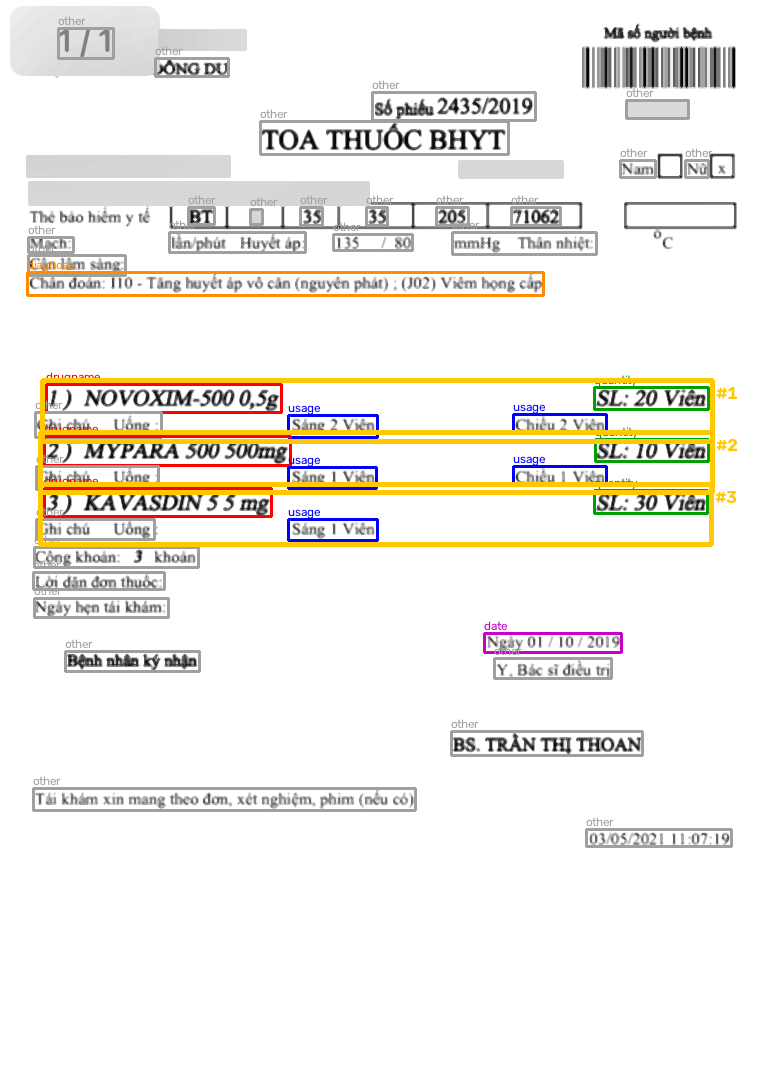
\includegraphics[width=0.5\linewidth]{common/pipeline_example.png}
\caption{Kết quả đầu-cuối trên một ảnh mẫu VAIPE sau tiền xử lý. Khung màu theo lớp YOLO gồm đỏ (\texttt{drugname}), xanh lá (\texttt{quantity}), xanh dương (\texttt{usage}), cam (\texttt{diagnose}), tím (\texttt{date}) và xám (\texttt{other}). Khung vàng \#1 đến \#3 là ba khoản thuốc sau bước ghép khoản. Cả ba khoản đúng tên, số lượng và cách dùng, lỗi duy nhất là mã bệnh ``I10'' bị đọc thành ``110'', cùng kiểu lỗi với Hình~\ref{fig:c3err}(c).}\label{fig:example}
\end{figure}

\begin{figure}[H]
\centering
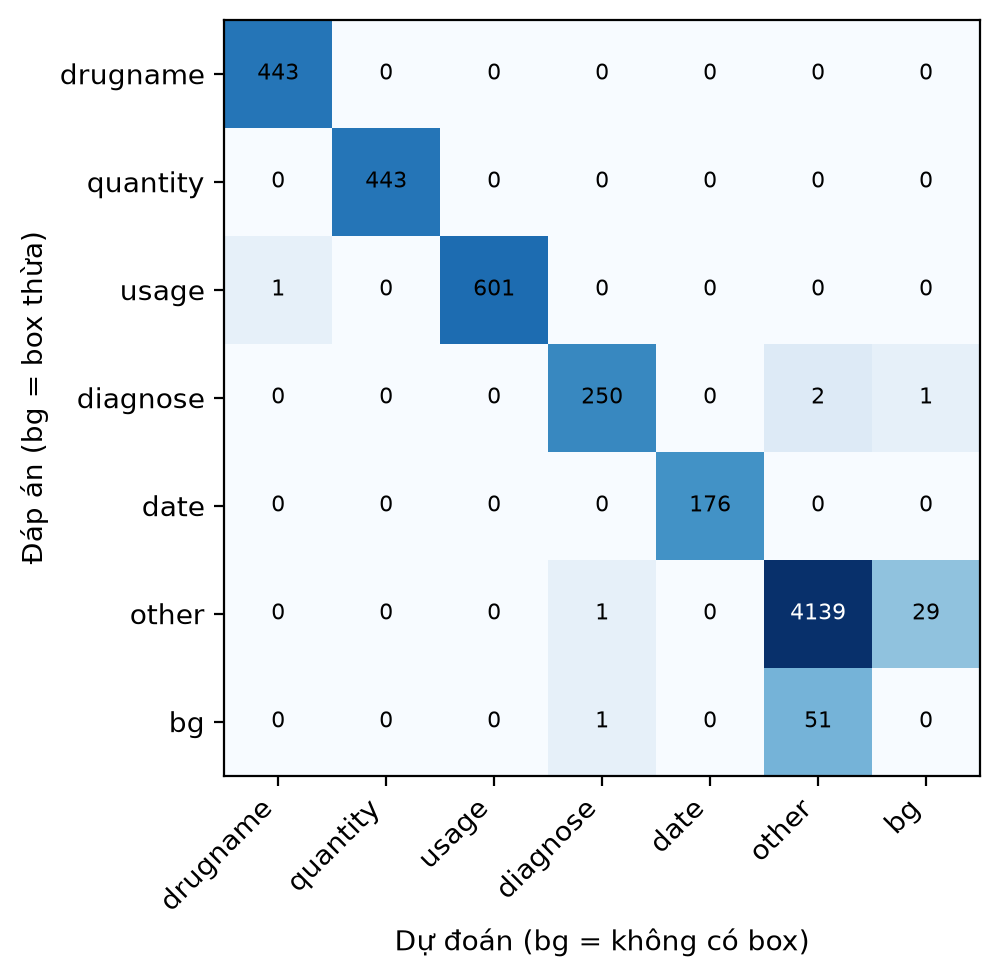
\includegraphics[width=0.42\linewidth]{e_b_detection/b2_confusion.png}
\caption{Ma trận nhầm lẫn của YOLOv8s trên 176 ảnh kiểm tra với IoU $\ge0{,}5$. Hàng \texttt{bg} là khung dự đoán thừa, cột \texttt{bg} là vùng chuẩn bị bỏ sót. Lỗi chủ yếu là sót hoặc thừa khung \texttt{other}; rất ít vùng bị nhầm giữa các lớp.}\label{fig:confusion}
\end{figure}

\begin{figure}[H]
\centering
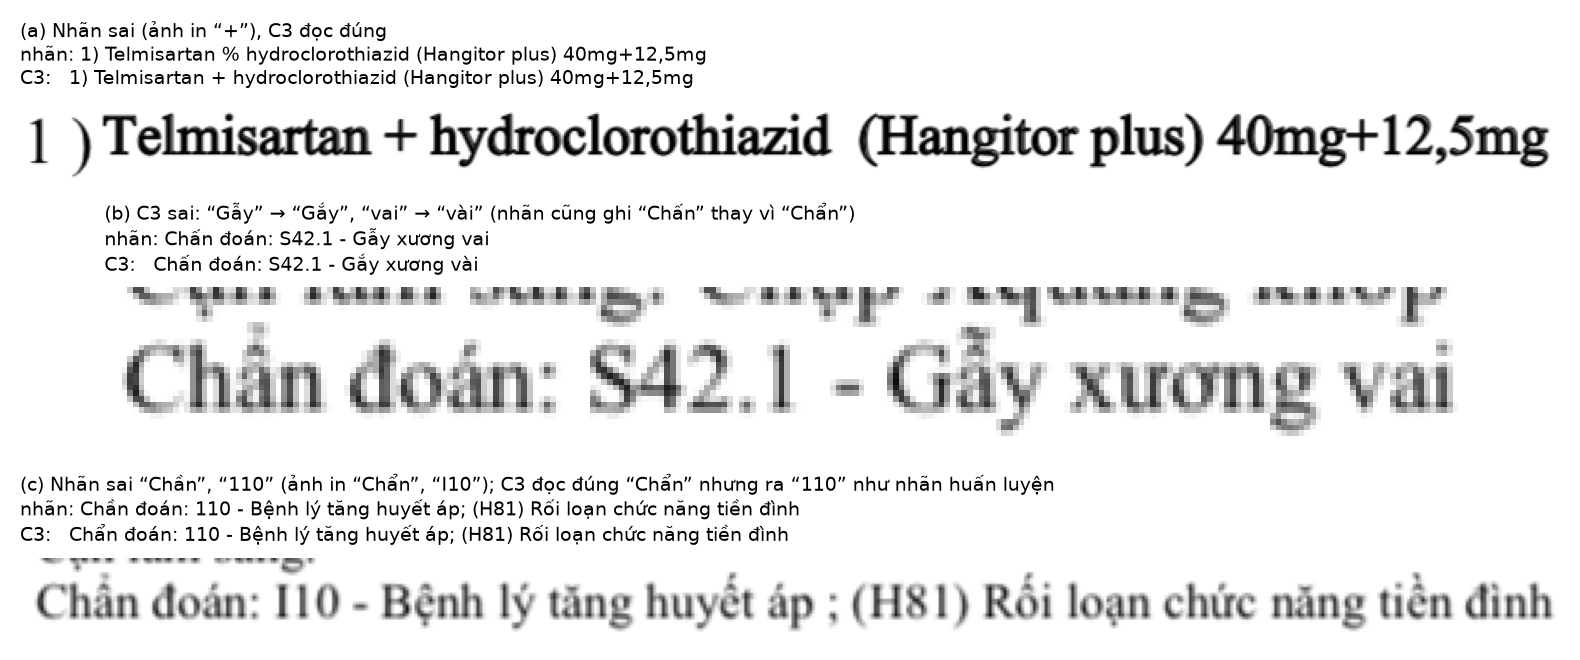
\includegraphics[width=0.9\linewidth]{e_c1_ocr/c3_errors.png}
\caption{Ba vùng VietOCR tinh chỉnh đọc khác nhãn. (a) Nhãn sai, mô hình đọc đúng. (b) Mô hình sai dấu từ ``Gẫy'' thành ``Gắy'' và từ ``vai'' thành ``vài''. (c) Nhãn huấn luyện ghi ``110'' thay vì ``I10'' và mô hình đọc theo nhãn.}\label{fig:c3err}
\end{figure}

\subsection*{Minh họa tiền xử lý}
Hình~\ref{fig:levels} là ba mức suy giảm dùng trong thí nghiệm độ bền, Hình~\ref{fig:shadow} minh họa bước khử bóng, và Hình~\ref{fig:asteps} là một ảnh suy giảm nặng qua đủ năm bước tiền xử lý.

\begin{figure}[H]
\centering
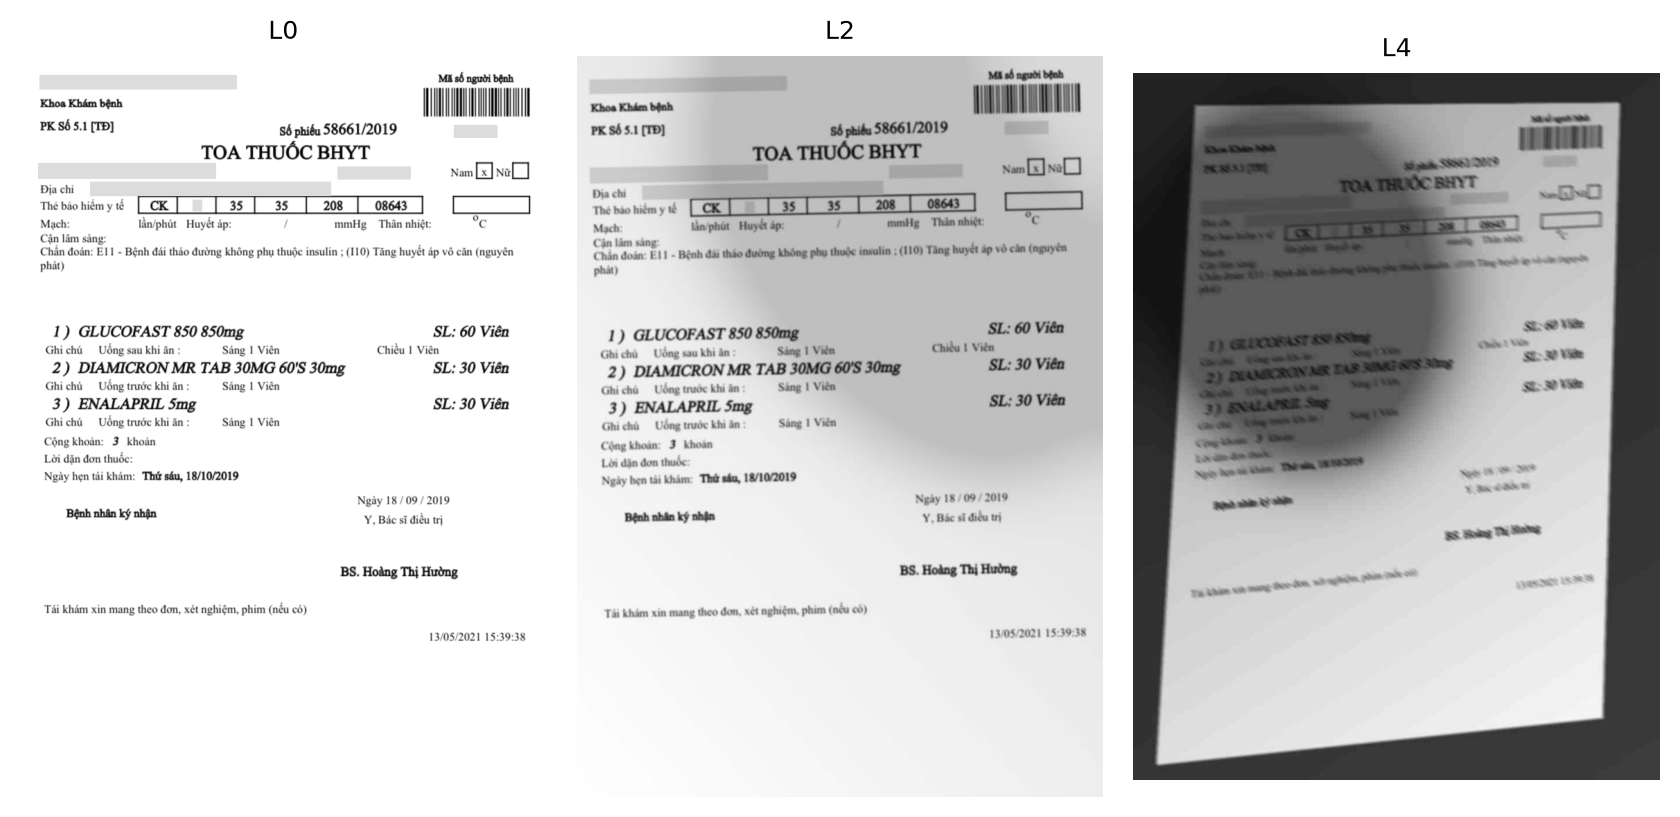
\includegraphics[width=0.95\linewidth]{fig_enhance/a_levels.png}
\caption{Một ảnh kiểm tra ở ba mức suy giảm là ảnh gốc, suy giảm nhẹ và suy giảm nặng.}\label{fig:levels}
\end{figure}

\begin{figure}[H]
\centering
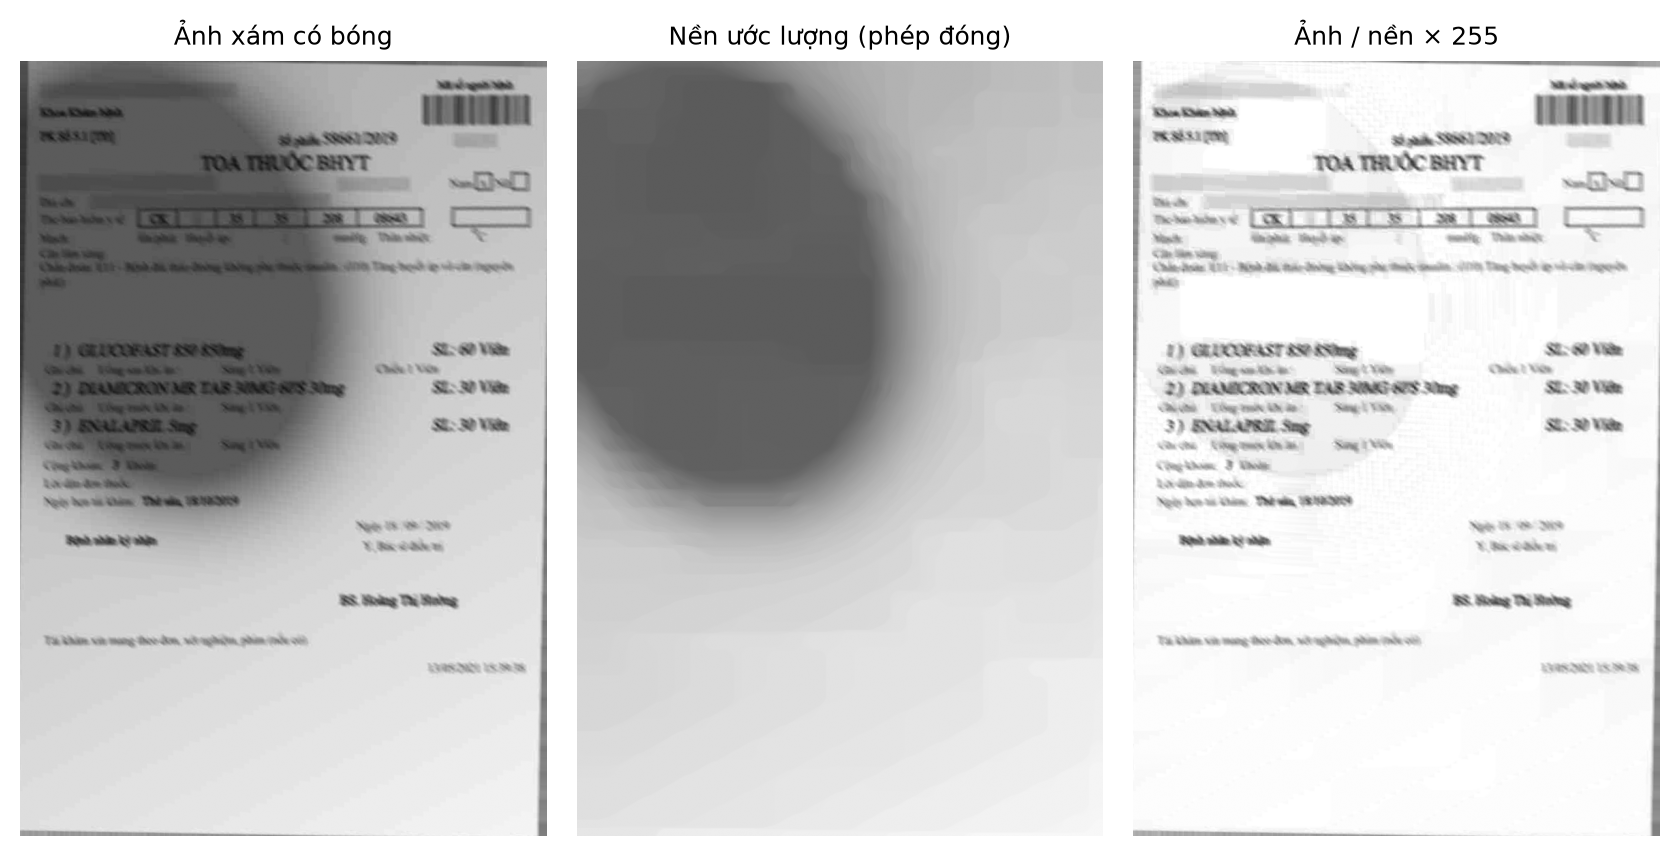
\includegraphics[width=0.95\linewidth]{fig_enhance/a_shadow.png}
\caption{Khử bóng: ảnh xám có bóng, nền ước lượng bằng phép đóng $81\times81$, ảnh sau khi chia cho nền.}\label{fig:shadow}
\end{figure}

\begin{figure}[H]
\centering
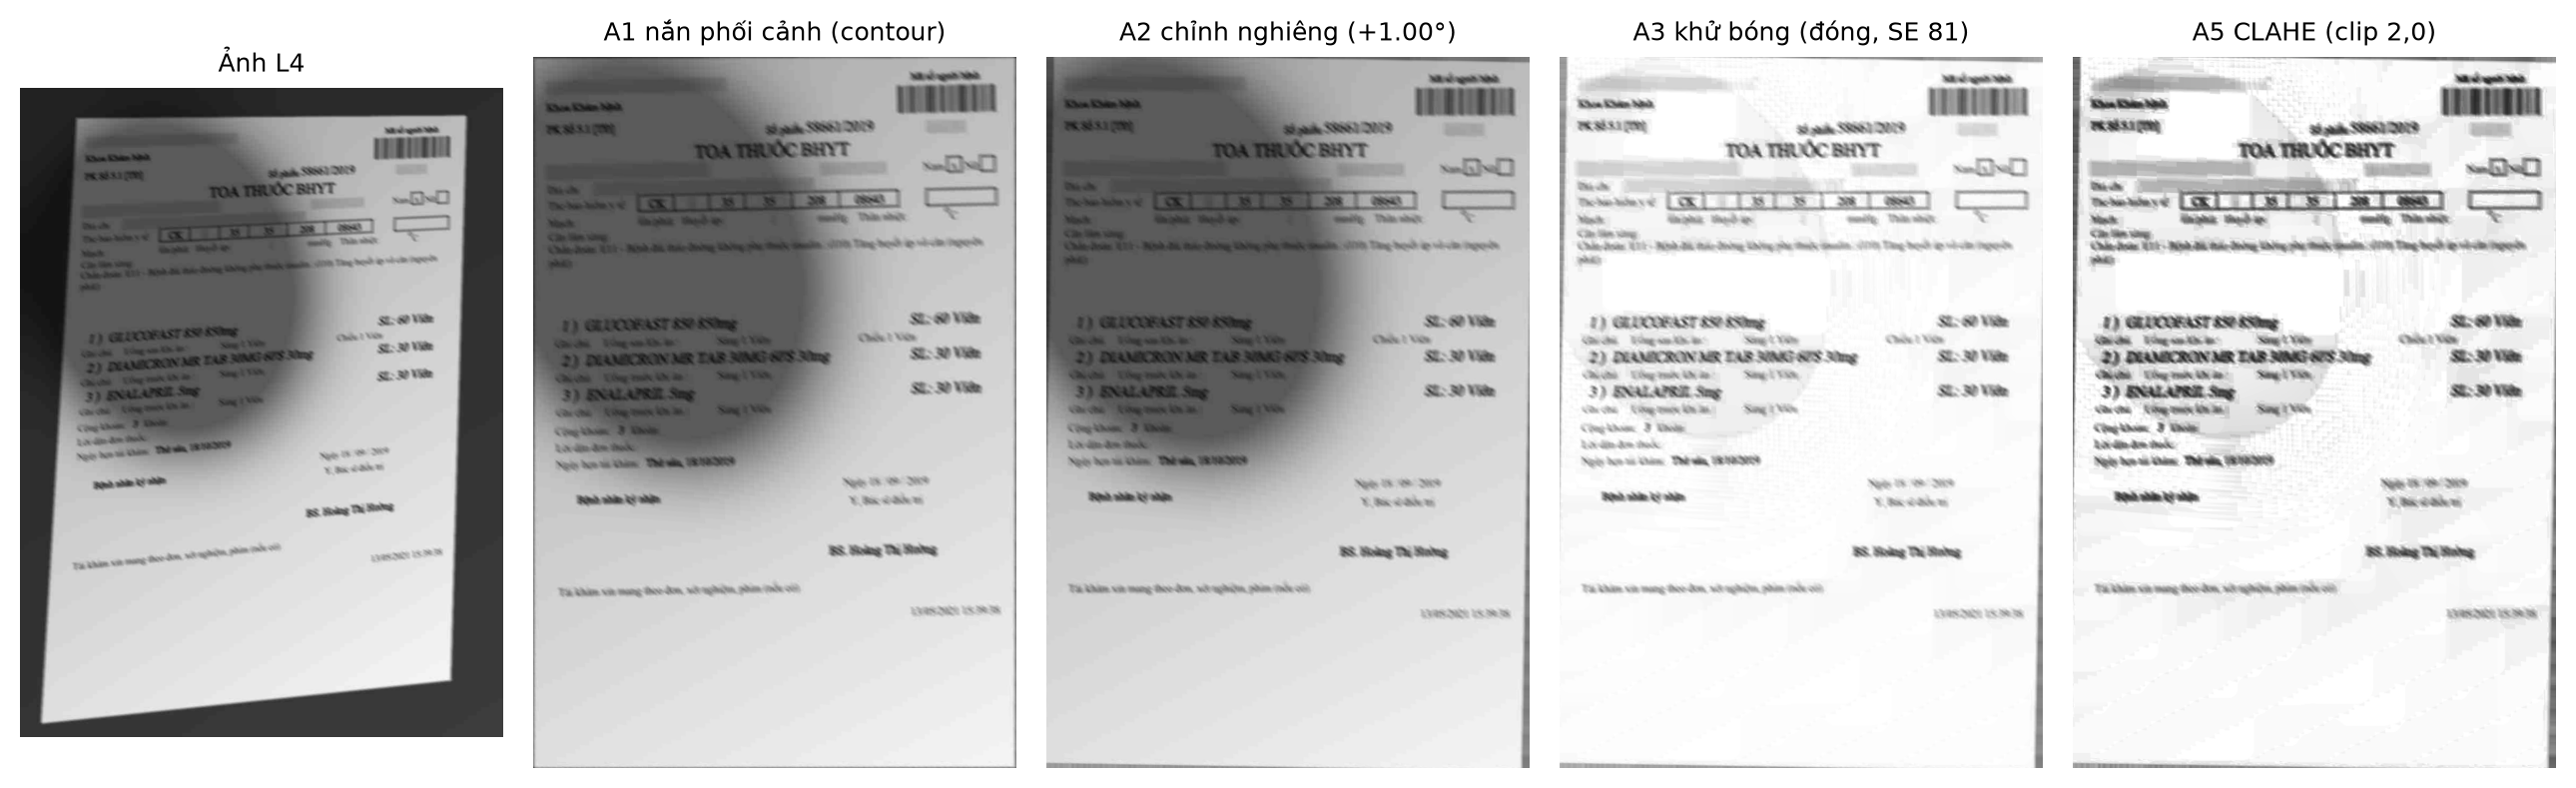
\includegraphics[width=\linewidth]{fig_enhance/a_steps.png}
\caption{Ảnh suy giảm nặng qua các bước tiền xử lý. Nắn phối cảnh và chia nền loại bỏ nền bàn tối và vùng bóng, nhưng độ mờ vẫn còn và CLAHE làm xuất hiện vài vệt khối ở vùng nền.}\label{fig:asteps}
\end{figure}
